\documentclass[11pt]{jarticle}

\usepackage[dvipdfmx]{graphicx}
\usepackage{listings}

\lstset{
    basicstyle={\ttfamily\small}, %書体の指定
    frame=tRBl, %フレームの指定
    framesep=10pt, %フレームと中身(コード)の間隔
    breaklines=true, %行が長くなった場合の改行
    linewidth=16cm, %フレームの横幅
    lineskip=-0.5ex, %行間の調整
    tabsize=2 %Tabを何文字幅にするかの指定
}

\setlength{\oddsidemargin}{-6.35mm}
\setlength{\textwidth}{171.9mm}

\begin{document}

\title{画像処理実験 第4回}
\author{09430565\\大橋虎ノ介}
\date{\number\year 年\number\month 月\number\day 日}
\maketitle

\section{概要}

 今回の実験では,特徴点の自動検出を行う.
具体的には,横方向と縦方向で色の変化の大きさを計算し,色の変化が大きい画素をが特徴点としてふさわしいものとする.

\section{CPUで計算を行うプログラム}

各画素の特徴点らしさを格納するためのMatrix型とMatrix型の領域を確保するMatrixAlloc関数を以下のように定義した.

\begin{lstlisting}
typedef struct _Matrix {
    unsigned char* data;
    int H,W;
} Matrix;

Matrix* MatrixAlloc(int w, int h) {
    Matrix* mt = (Matrix*)malloc(sizeof(Matrix));
    mt->W = w;
    mt->H = h;
    mt->data = (unsigned char*)malloc(w * h);
    return mt;
}
\end{lstlisting}

次に色の変化量を計算するImageFeature関数と2つの固有値の内小さい方を計算するCalcSmallerEigenValue関数を以下のように定義した.

\begin{lstlisting}
double CalcSmallerEigenValue(double a, double b, double c, double d) {
    double x = ((a + d) - sqrt((a + d) * (a + d) 
                - 4 * (a * d - b * c))) / 2;
    return x;
}

void ImageFeature(Matrix* im2, Image* im) {
    int x, y, u, v, W = 7;
    double ix, iy;
    for (y = W + 1; y < im->H - W - 1; y++) for (x = W + 1; x < im->W - W - 1; x++) {
        double ixx, ixy, iyy;
        ixx = iyy = ixy = 0;
        for (v = -W; v <= W; v++) for (u = -W; u <= W; u++) {
            ix = IElem(im, x + u + 1, y + v, 1) - IElem(im, x + u - 1, y + v, 1);
            iy = IElem(im, x + u, y + v + 1, 1) - IElem(im, x + u, y + v - 1, 1);
            ixx += ix * ix;
            ixy += ix * iy;
            iyy += iy * iy;
        }
        DElem(im2, x, y) = CalcSmallerEigenValue(ixx, ixy, ixy, iyy);
    }
}
\end{lstlisting}

このプログラムで左図の画像を計算すると右図の画像が得られた.

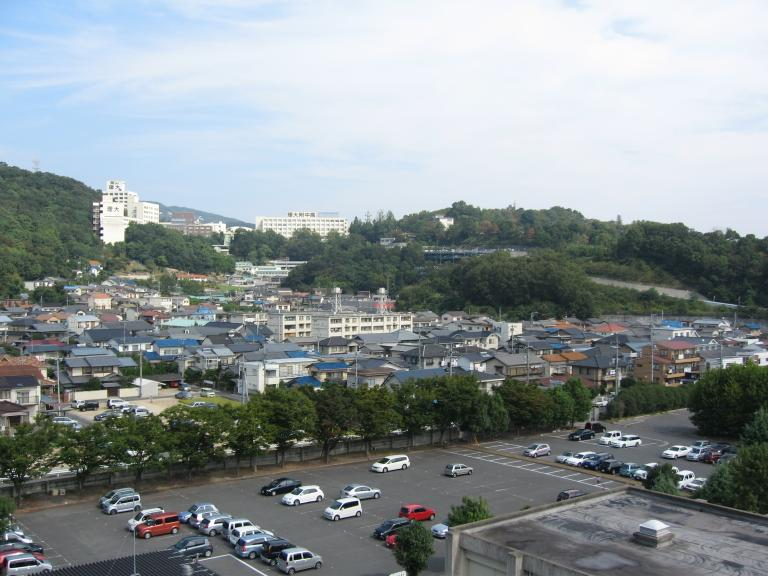
\includegraphics[scale=.3]{./img/0.jpg}
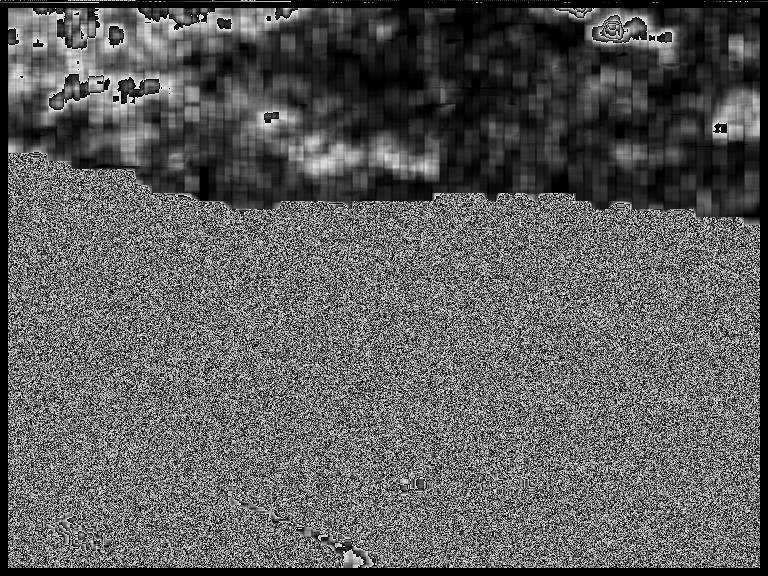
\includegraphics[scale=.4]{./img/out.jpg}

\section{効率化}

短径領域での和を2段階に分けることで効率化を図る.
ソースコードを以下に示す.

\begin{lstlisting}
void ImageFeature(Matrix* im2, Image* im) {
    int x, y, u, v, W = 7;
    double ix, iy;
    Matrix* tmpxx,*tmpxy,*tmpyy;
    tmpxx = MatrixAlloc(im2->W, im2->H);
    tmpxy = MatrixAlloc(im2->W, im2->H);
    tmpyy = MatrixAlloc(im2->W, im2->H);
    for (y = W + 1; y < im->H - W - 1; y++) for (x = W + 1; x < im->W - W - 1; x++) {
        double ixx, ixy, iyy;
        ixx = iyy = ixy = 0;
        for (u = -W; u <= W; u++) {
            ix = IElem(im, x + u + 1, y, 1) - IElem(im, x + u - 1, y, 1);
            iy = IElem(im, x + u, y + 1, 1) - IElem(im, x + u, y - 1, 1);
            ixx += ix * ix;
            ixy += ix * iy;
            iyy += iy * iy;
        }
        DElem(tmpxx, x, y) = ixx;
        DElem(tmpxy, x, y) = ixy;
        DElem(tmpyy, x, y) = iyy;
    }

    for (y = W + 1; y < im->H - W - 1; y++) for (x = W + 1; x < im->W - W - 1; x++) {
        double ixx, ixy, iyy;
        ixx = iyy = ixy = 0;
        for (v = -W; v <= W; v++) {
            ixx += DElem(tmpxx, x, y + v);
            ixy += DElem(tmpxy, x, y + v);
            iyy += DElem(tmpyy, x, y + v);
        }
        DElem(im2, x, y) = CalcSmallerEigenValue(ixx, ixy, ixy, iyy);
    }
}
\end{lstlisting}

改良することで235msecから35msecまで高速化できた.

\section{考察}

今回の実験では,各画素の色の変化の大きさを調べることで,特徴点になりうるかどうかを調べる処理を実装した.
プログラムを実装し,得られた画像は実験Bのページの「特徴点らしさ」画像とは少し違うものになった.
原因は現時点では解明できなかった.

また,追加課題として,短径領域での和の処理の高速化を行った.
15*15回の要素の足し算を2段階に分けることにより,15+15回の足し算に減らすものだ.
改良することによって,235msecから35msec,実行時間を30/225(15+15 / 15*15)にすることができた.

\end{document}
